%****************************************************************************%
%* Resources allocation                                                     *%
%*                                                                          *%
%* Author(s):                                                               *%
%* - Abdelkader AMAR (Abdelkader.Amar@ens-lyon.fr)                          *%
%* - David LOUREIRO (David.Loureiro@ens-lyon.fr)                            *%
%*                                                                          *%
%* $LICENSE$                                                                *%
%****************************************************************************%
%* $Id: GUM_resources.tex,v 1.4 2007/11/29 16:03:21 dloureir Exp $
%* $Log: GUM_resources.tex,v $
%* Revision 1.4  2007/11/29 16:03:21  dloureir
%* typo corrections
%*
%* Revision 1.3  2007/11/08 16:28:54  dloureir
%* Adding some corrections and updates
%*
%* Revision 1.2  2007/11/08 11:31:14  dloureir
%* Correcting the headers
%*
%****************************************************************************%
\chapter{Resources allocation}

\section{Using OAR interface}
\label{sec:oar}

The most used operation is probably the resources allocation. In \gfk,
this operation can be done by the OAR system. \grudu provides an easy way
to manipulate OAR (either the OAR1 or OAR2 versions). The resources allocation window on
Figure \ref{fig:cfg_tab1} shows a map of France with \gfk sites~\footnote{You
can allocate resources only on enabled sites} and jobs characteristics (time,
queue, oargridsub behaviour, the script to launch). 

These information are presented on the first tab of the
window. The second tab provides the definition of the properties for the
different sites.

Since some sites include more than one cluster, you have to click first on the
site, and then select the number of desired nodes for each cluster or you can
specify that you do not care where they are located).
When selecting resources numbers, the map displays the total number of requested
resources for each site\footnote{When the mouse is over the site box, a tooltip
will tell you the repartition of the nodes you may want to reserve}. Jobs characteristics
are:
\begin{itemize}
  \item Time parameters: date and reservation walltime. The starting time can
  be specified manually, or through the use of a calendar for the day and
  through boxes where you can specify the hour, the minute and the second. For
  the walltime you have to define the number of hours and the minutes of your reservation.
  \item Queue: default, deploy (for KaDeploy) or \textit{allow\_classic\_ssh}
  \footnote{specific for OAR2 but corresponds to default for OAR1}.
  \item OARGridSub behaviour: the user can specify if the reservation should be
  done with the OARGridSub behaviour, i.e. when the user chooses to realize
  several reservations on different sites, if one fails, all the previous
  successful reservations are deleted.
  \item A script to launch: The user can specify a script that will be launched
  in order to be executed on the reserved nodes. The reservation will be stopped
  when the script ends.
\end{itemize}

\begin{figure}[H]
\centering
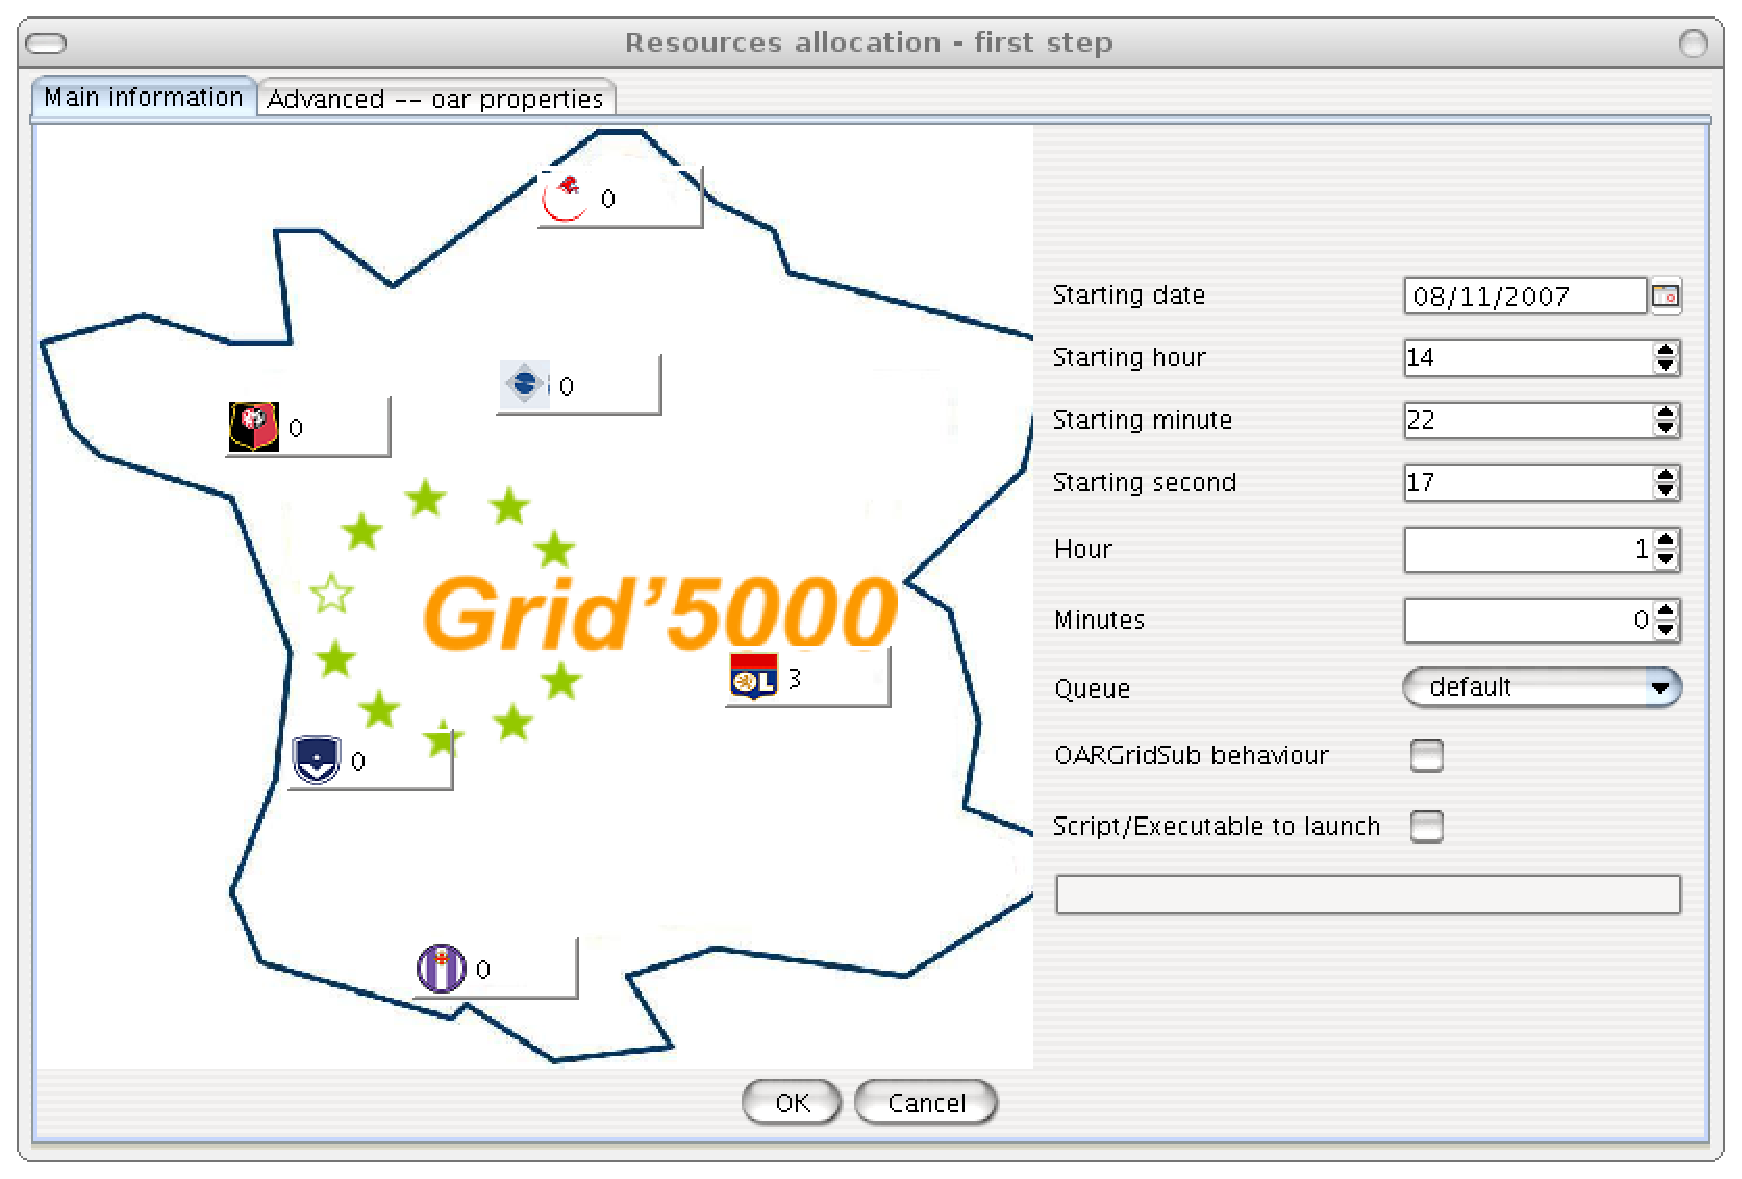
\includegraphics[width=0.6\linewidth]{figures/GRUDU_allocation_1.eps}
\caption{Resources allocation frame -- Main panel}
\label{fig:cfg_allocation1}
\end{figure}

Concerning the second tab of the window presented on Figure \ref{fig:cfg_tab2},
it allows the user to define the OAR properties that will be used for
 the reservation.
 
\begin{figure}[H]
\centering
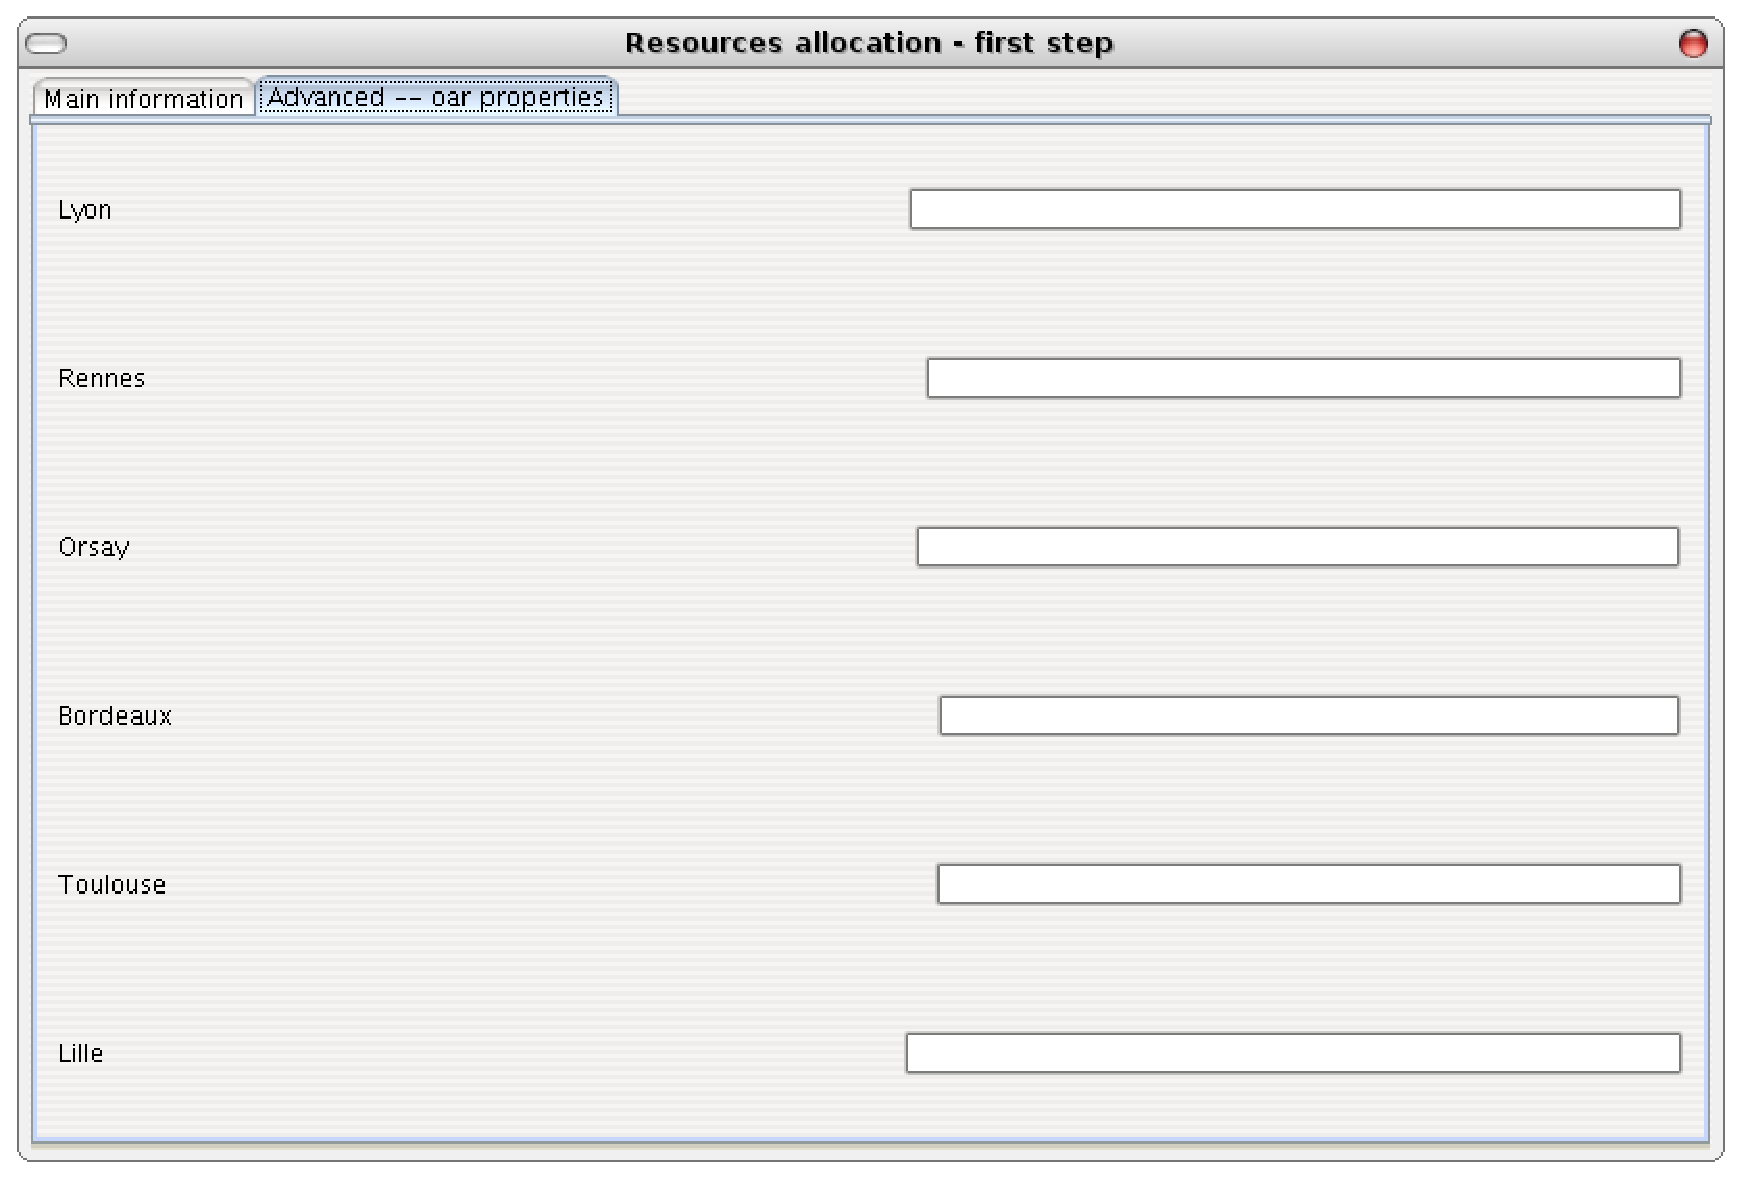
\includegraphics[width=0.6\linewidth]{figures/GRUDU_allocation_2.eps}
\caption{Resources allocation frame -- OAR properties for the reservation}
\label{fig:cfg_allocation2}
\end{figure}

After the reservation, a status frame summarizes the information about the
success (or not) of your jobs submission.

\begin{figure}[H]
\centering
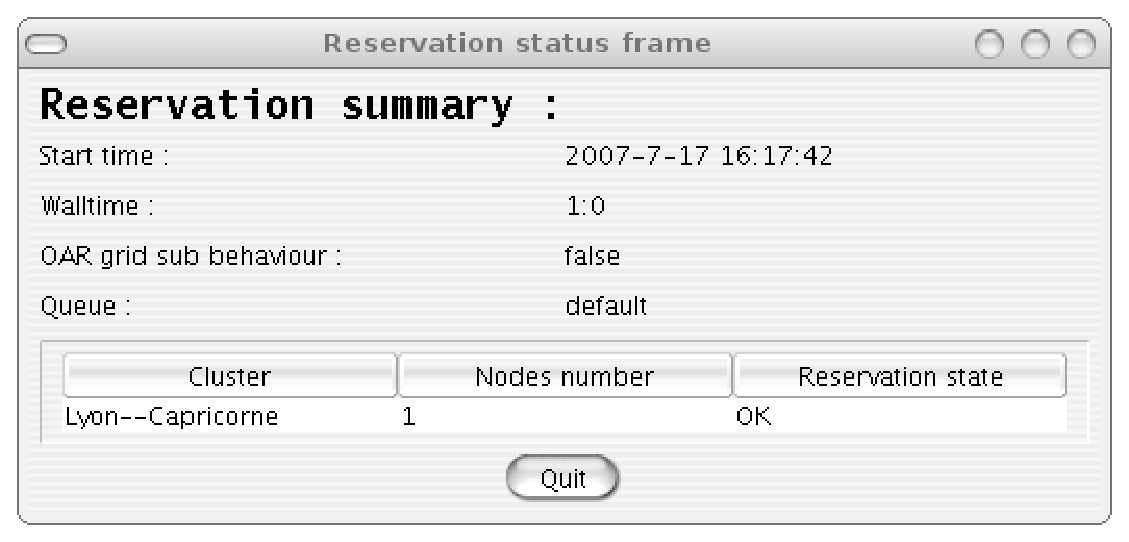
\includegraphics[width=0.6\linewidth]{figures/GRUDU_reservation1.eps}
\caption{Resources allocation frame -- Reservation status}
\label{fig:reservation_status}
\end{figure}

%******************************************%